\title{Lecture 9\\Representation of Logical Knowledge}

\begin{frame}
	\titlepage
\end{frame}

\begin{frame}{\\Lecture outline}
	\topline
	\justifying
	Formal logical languages. Alphabet and syntax of SCL. Predicates and Boolean functions. Logical connectives (operators), truth tables. Logical formulas, equivalent logical formulas, logical laws. Classes of logical formulas. Quantifiers and duality laws. Bound and free variables. Open and closed formulas. Representation in a knowledge base.
\end{frame}

\begin{frame}{\\Formal language}
	\topline
	\textbf{\textit{A formal language}} is a set of finite words (strings) over a finite alphabet.
	\bigskip
	If \textit{L} is a formal language and \textit{A} is its alphabet, then $L \subseteq A^*$, where $A^*$ is the closure operation on the set \textit{A}.
	\bigskip
	Formal logical languages include the language of \textbf{propositional logic} and the language of \textbf{first-order predicate logic}.
\end{frame}

\begin{frame}{\\The formal logical language SCL}
	\topline
	\justifying
	The formal logical language SCL is a sublanguage of SC, defined by a particular set of special key nodes whose semantics must be known and agreed upon in advance.
	\bigskip
	SCL is a set-theoretic logical language. It interprets logical connectives and quantifiers through sets, tuples, attributes and relations, treating formal theories and non-atomic logical formulas as relational structures over propositions.
\end{frame}

\iffalse
\begin{frame}{\\The formal logical language SCL}
	\topline
	\justifying
	SCL is a sublanguage of SC and has two variants:
	\begin{textitemize}
		\item{the linear variant, SCLs (Semantic Code Logic string);}
		\item{the graphical variant, SCLg (Semantic Code Logic graphical). }
	\end{textitemize}
	The main difference between SCLs and a classical logical language is the notation for atomic logical formulas. An atomic logical formula in SCLs is an SCs text enclosed in square brackets. Non-atomic (compound) logical formulas in SCLs are constructed in the same way as in classical logical languages.
\end{frame}
\fi

\begin{frame}{\\Predicate. Boolean function}
	\topline
	\textbf{A predicate} is a function with codomain $\{\top, \bot\}$ and domain $M^n$, where $M$ is the set of objects in the subject domain.\\
	\textbf{A Boolean function} is a function with domain $B^n$ and codomain $B$, where $B = \{\top, \bot\}$.\\
	\textbf{A Boolean function} is specified by a finite set of values and can therefore be represented by a truth table.
\end{frame}

\begin{frame}{\\Truth table}
	\topline
	\justifying
	\textbf{A truth table} is a table that relates every possible combination of the logical variables in a logical function to the value of that function.\\
	\vspace{5mm}
	\begin{center}
		\begin{tabular}{|c|c|c|}
			\hline
			$X$ & $Y$ & $F(X,Y)$\\
			\hline
			$0$ & $0$ & $0$\\
			\hline
			$0$ & $1$ & $1$\\
			\hline
			$1$ & $0$ & $1$\\
			\hline
			$1$ & $1$ & $0$\\
			\hline
		\end{tabular}
	\end{center}
\end{frame}

\begin{frame}{\\Proposition}
	\topline
	\justifying
	\begin{SCn}
		\scnheader{proposition}
		\scntext{explanation}{A \textbf{\textit{proposition}} is understood as a \textit{structure} (containing \textit{sc-constants} from a subject domain and/or \textit{sc-variables}) or a \textit{logical connective} that can be interpreted as true or false within a \textit{subject domain}.}
		\begin{scnreltoset}{\textit{partition}}
			\scnitem{atomic proposition}
			\scnitem{non-atomic proposition}
		\end{scnreltoset}
		\begin{scnreltoset}{\textit{partition}}
			\scnitem{factual proposition}
			\scnitem{logical formula}
		\end{scnreltoset}
	\end{SCn}
\end{frame}

\begin{frame}{\\Proposition}
	\topline
	\justifying
	\\
The truth of a \textbf{\textit{proposition}} is specified by indicating that the sign of this proposition belongs to the \textit{formal theory} corresponding to the given \textit{subject domain}. Its falsity is specified by indicating that the sign of the \textit{negation*} of this proposition belongs to that \textit{formal theory}.\\
Explicitly specified non-membership of a \textbf{\textit{proposition}} in a \textit{formal theory} may indicate either its falsity within that theory (if specified as above), or that the  \textbf{\textit{proposition}} is not considered at all in that \textit{formal theory} (for example, it uses concepts that do not belong to that \textit{subject domain}).\\
The same \textbf{\textit{proposition}} may be true within one \textit{formal theory} and false within another.
\end{frame}

\begin{frame}{\\Proposition of a formal theory}
	\topline
	\justifying
	\begin{SCn}
		\scnheader{proposition of a formal theory\scnrolesign}
		\scniselement{non-basic concept}
		\begin{scnreltoset}{partition}
			\scnitem{true proposition\scnrolesign}
			\scnitem{false proposition\scnrolesign}
			\scnitem{fuzzy proposition\scnrolesign}
			\scnitem{meaningless proposition\scnrolesign}
		\end{scnreltoset}
	\end{SCn}
\end{frame}

\begin{frame}{\\ \small{True proposition. False proposition.}}
	\topline
	\justifying
	\begin{SCn}
		\scnheader{true proposition\scnrolesign}
		\scnidtf{proposition that is true within a given formal theory\scnrolesign}
		\scnidtf{proposition whose sign belongs to a given formal theory\scnrolesign}
		\scnheader{false proposition\scnrolesign}
		\scnidtf{proposition that is false within a given formal theory\scnrolesign}
		\scnidtf{proposition whose negation sign belongs to a given formal theory\scnrolesign}
	\end{SCn}
\end{frame}

\begin{frame}{\\ \small{Fuzzy proposition. Meaningless proposition}}
	\topline
	\justifying
	\begin{SCn}
		\small{
			\scnheader{fuzzy proposition\scnrolesign}
			\scnidtf{hypothetical proposition\scnrolesign}
			\scnidtf{proposition that may be true or false within a given formal theory\scnrolesign}
			\scnidtf{proposition that is true or false within a given formal theory with a certain probability\scnrolesign}
			\scnheader{meaningless proposition\scnrolesign}
			\scnidtf{proposition that is meaningless within a given formal theory\scnrolesign}
			\scnidtf{proposition that is not considered within a given formal theory\scnrolesign}
			\scntext{explanation}{A proposition is meaningless within a given formal theory if an \textit{atomic proposition} within it (or the proposition itself, if atomic) contains an \textit{sc-constant} that is not an element of the subject domain described by that \textit{formal theory}.}}
	\end{SCn}
\end{frame}

\begin{frame}{\\ \small{Atomic proposition. Non-atomic proposition}}
	\topline
	\justifying
	\footnotesize{
		\begin{SCn}
			\scnheader{atomic proposition}
			\scnsubset{structure}
			\begin{scnreltoset}{partition}
				\scnitem{atomic factual proposition}
				\scnitem{atomic logical formula}
			\end{scnreltoset}
			\scntext{explanation}{\textbf{\textit{atomic proposition}} is a \textit{proposition} that contains at least one \textit{sc-element} that is not the sign of another \textit{proposition}.}
			\scnheader{non-atomic proposition}
			\scntext{explanation}{\textbf{\textit{non-atomic proposition}} is a \textit{proposition} that consists only of the signs of other \textit{propositions}.
We cannot speak of the truth or falsity of a \textbf{\textit{non-atomic proposition}} within a \textit{formal theory} when the truth or falsity of any of its elements cannot be established within the same \textit{formal theory}.}
		\end{SCn}
	}
\end{frame}

\begin{frame}{\\Factual proposition}
	\topline
	\justifying
	\begin{SCn}
		\scnheader{factual proposition}
		\scnsuperset{atomic factual proposition}
	\end{SCn}

	A \textbf{\textit{factual proposition}} is understood as:
	\begin{textitemize}
		\item \textit{atomic proposition} that contains no \textit{sc-variable}
		\item \textit{non-atomic proposition} all of whose elements are also \textbf{\textit{factual propositions}}
	\end{textitemize}

\end{frame}

\begin{frame}{\\Logical formula}
	\topline
	\justifying
	\footnotesize
	\vspace{10mm}

	A \textbf{logical formula} is understood as:
	\begin{textitemize}
		\item \textit{atomic proposition} that contains at least one \textit{sc-variable};
		\item \textit{non-atomic proposition} at least one of whose elements is a \textbf{\textit{logical formula}}.
	\end{textitemize}

	\begin{SCn}
		\scnheader{logical formula}
		\begin{scnreltoset}{partition}
			\scnitem{atomic logical formula}
			\scnitem{non-atomic logical formula}
		\end{scnreltoset}
		\begin{scnreltoset}{partition}
			\scnitem{open logical formula}
			\scnitem{closed logical formula}
		\end{scnreltoset}
	\end{SCn}
\end{frame}

\begin{frame}{\\Logical connectives (operators)}
	\topline
	\justifying
	\begin{SCn}
		\scnheader{logical connective*}
		\scnidtf{non-atomic logical formula}
		\scnidtf{logical operator*}
		\scnidtf{propositional connective*}
		\scniselement{class of tuples of different cardinalities}
		\scnrelto{family of subsets}{non-atomic proposition}
		\scntext{explanation}{\textbf{\textit{logical connective*}} is a relation (a class of tuples) whose tuples are \textit{propositions}.
			\textbf{\textit{logical connective*}} is a \textit{relation} whose domain is the set of \textit{propositions}; this relation and some of its subsets may be \textit{classes of tuples of different cardinalities}.}
	\end{SCn}
\end{frame}

\begin{frame}{\\Conjunction}
	\topline
	\justifying
	\small{
		\begin{SCn}
			\scnheader{conjunction*}
			\scnidtf{logical and*}
			\scnidtf{logical multiplication*}
			\scnsubset{logical connective*}
			\scniselement{undirected relation}
			\scniselement{class of tuples of different cardinalities}
			\scntext{explanation}{\textbf{\textit{conjunction*}} is a set of conjunctive \textit{propositions}, each of which is true within a \textit{formal theory} if and only if all its components are true within the same \textit{formal theory}.
			\textbf{\textit{conjunction*}} of atomic formulas can be replaced by an atomic formula obtained by uniting the original atomic formulas.}
		\end{SCn}
	}
\end{frame}

\begin{frame}{\\Conjunction}
	\topline
	\justifying
	\vspace{10mm}
	\begin{figure}[H]
		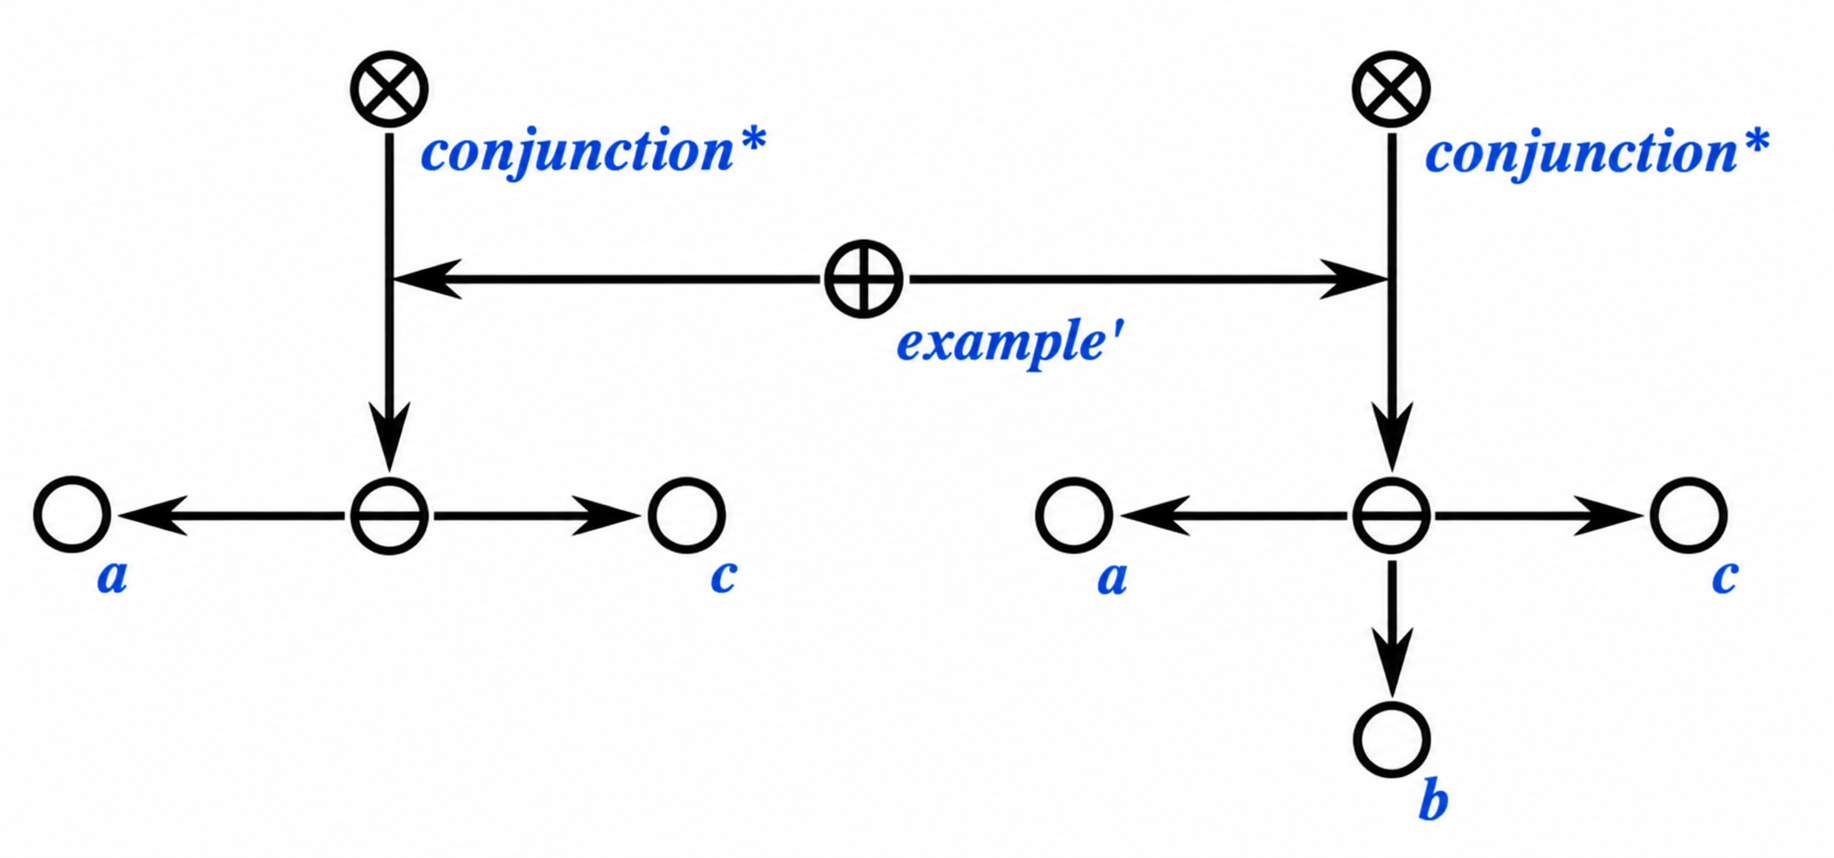
\includegraphics[width=301.5bp,height=141bp,keepaspectratio]{./figures/sd_logic/conjunction_en.png}
	\end{figure}
\end{frame}

\begin{frame}{\\Disjunction}
	\topline
	\justifying
	\small{
		\begin{SCn}
			\scnheader{disjunction*}
			\scnidtf{logical or*}
			\scnidtf{logical addition*}
			\scnidtf{inclusive or*}
			\scnsubset{logical connective*}
			\scniselement{undirected relation}
			\scniselement{class of tuples of different cardinalities}
			\scntext{explanation}{\textbf{\textit{disjunction*}} is a set of disjunctive \textit{propositions}, each of which is true within a \textit{formal theory} if and only if at least one of its components is true within the same \textit{formal theory}.}
		\end{SCn}
	}
\end{frame}

\begin{frame}{\\Disjunction}
	\topline
	\justifying
	\vspace{10mm}
	\begin{figure}[H]
		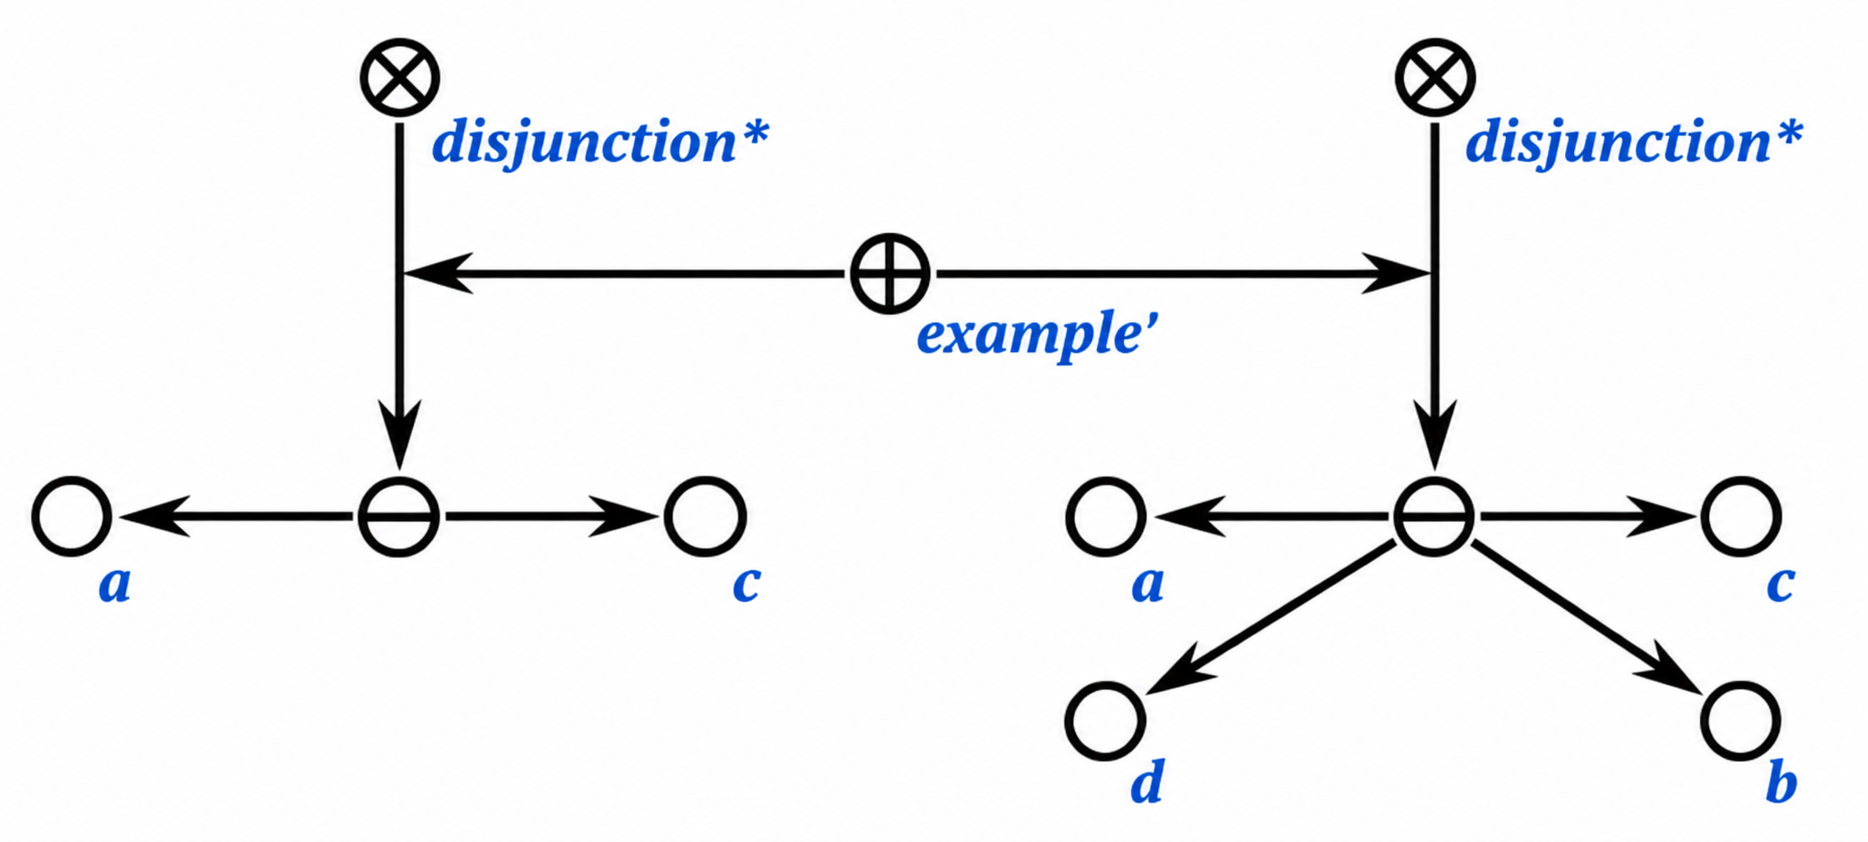
\includegraphics[width=296.25bp,height=133.5bp,keepaspectratio]{./figures/sd_logic/disjunction_en.png}
	\end{figure}
\end{frame}

\begin{frame}{\\Negation}
	\topline
	\justifying
	\begin{SCn}
		\scnheader{negation*}
		\scnsubset{logical connective*}
		\scnsubset{singleton}
		\scntext{explanation}{\textbf{\textit{negation*}} is a set of \textit{propositions} about negation, each of which is true within a \textit{formal theory} if and only if its sole element is false within the same \textit{formal theory}.}
	\end{SCn}
\end{frame}

\begin{frame}{\\Negation}
	\topline
	\justifying
	\vspace{10mm}
	\begin{figure}[H]
		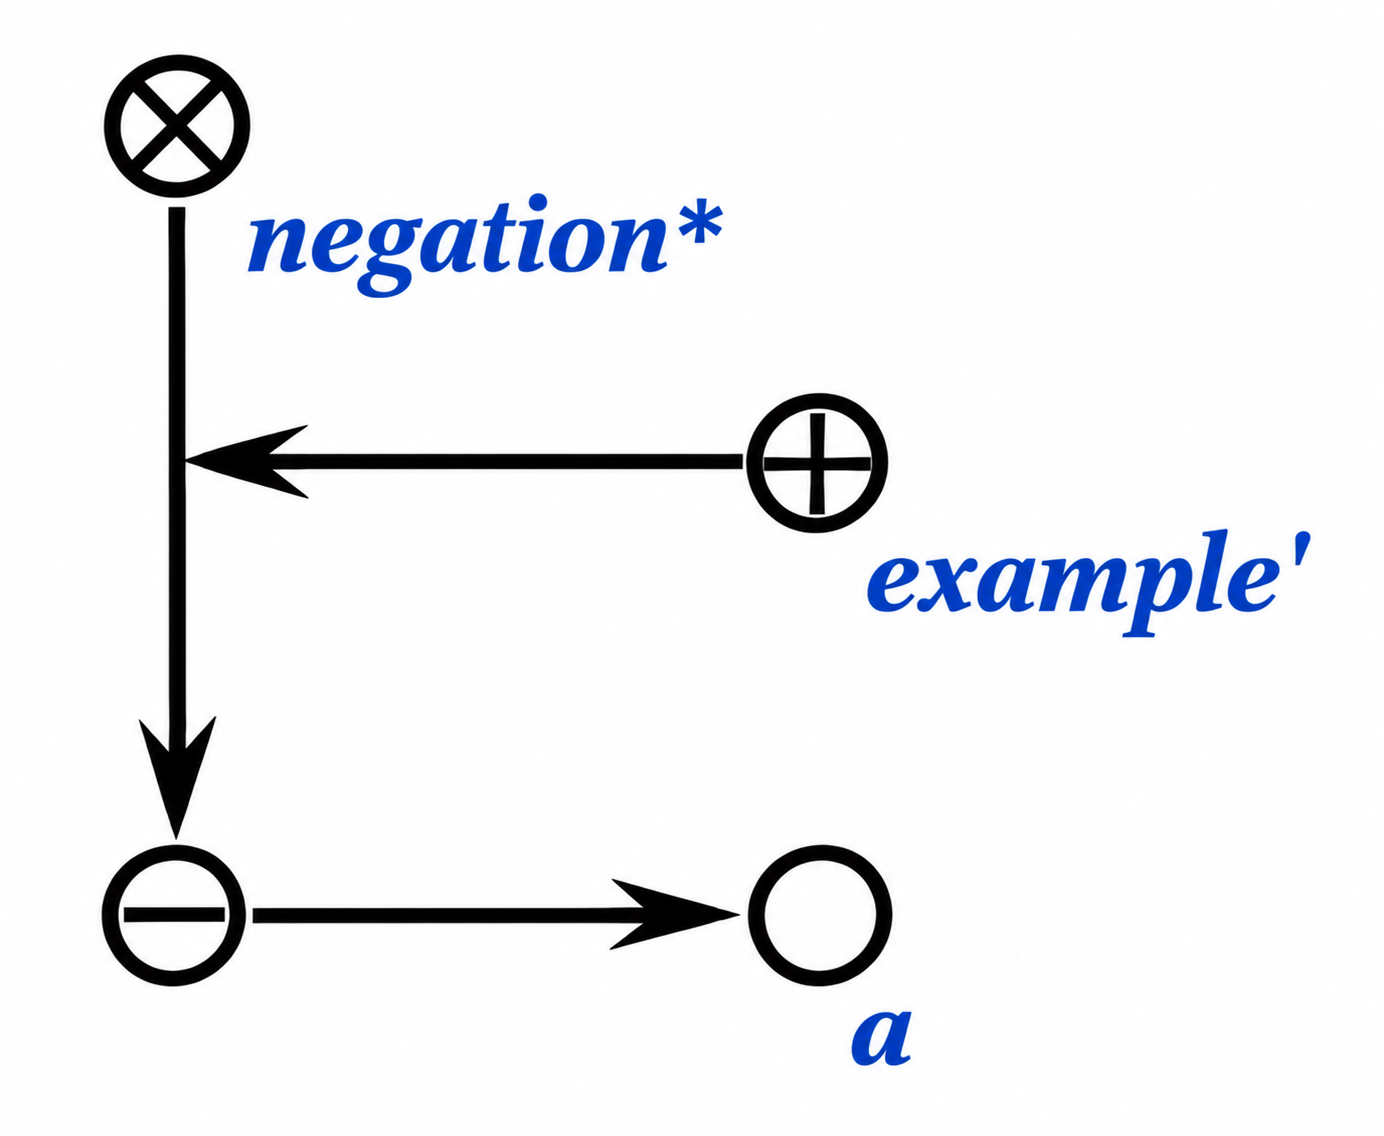
\includegraphics[width=121.5bp,height=99.75bp,keepaspectratio]{./figures/sd_logic/negation_en.png}
	\end{figure}
\end{frame}

\begin{frame}{\\Exclusive disjunction}
	\topline
	\justifying
	\begin{SCn}
		\scnheader{exclusive disjunction*}
		\scnidtf{addition modulo 2*}
		\scnidtf{exclusive or*}
		\scnidtf{alternative*}
		\scnsubset{logical connective*}
		\scniselement{undirected relation}
		\scniselement{class of tuples of different cardinalities}
		\scntext{explanation}{\textbf{\textit{exclusive disjunction*}} is a set of exclusively disjunctive \textit{propositions}, each of which is true within a \textit{formal theory} if and only if exactly one of its components is true within the same \textit{formal theory}.}
	\end{SCn}
\end{frame}

\begin{frame}{\\Exclusive disjunction}
	\topline
	\justifying
	\vspace{10mm}
	\begin{figure}[H]
		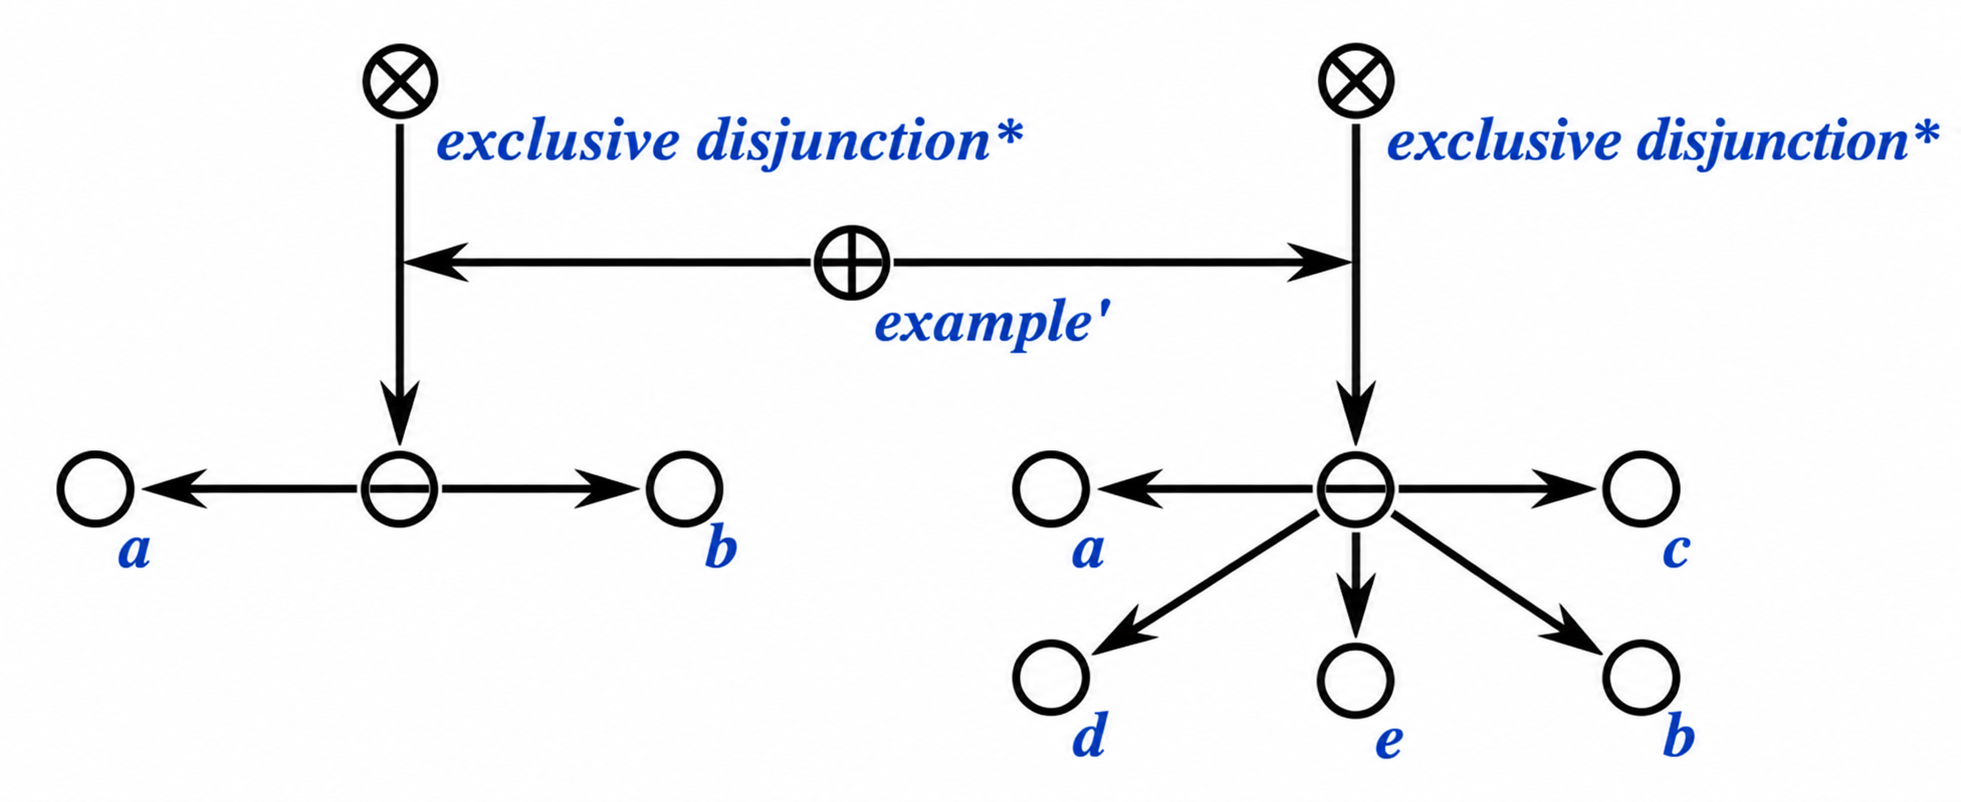
\includegraphics[width=337.5bp,height=138bp,keepaspectratio]{./figures/sd_logic/strictDisjunction_en.png}
	\end{figure}
\end{frame}

\begin{frame}{\\Implication}
	\topline
	\justifying
	\footnotesize{
		\begin{SCn}
			\scnheader{implication*}
			\scnidtf{logical implication*}
			\scnsubset{logical connective*}
			\scniselement{binary relation}
			\scniselement{directed relation}
			\scntext{explanation}{\textbf{\textit{implication*}} is a set of implicative \textit{non-atomic propositions}, each of which consists of a premise (the first component of the \textit{proposition}) and a conclusion (the second component of the \textit{proposition}).

Each implicative \textit{proposition} is false within a \textit{formal theory} when its premise is true and its conclusion is false within the same \textit{formal theory}. In all other cases, this \textit{proposition} is true.

By default, all variables occurring in both parts of a proposition about \textbf{\textit{implication*}} (or at least one of the \textit{subformulas*} of each part) are implicitly bound by a \textit{universal quantifier*}, provided that these variables are not bound by another \textit{quantifier} that is specified explicitly.}
		\end{SCn}
	}
\end{frame}

\begin{frame}{\\Implication}
	\topline
	\justifying
	\vspace{10mm}
	\begin{figure}[H]
		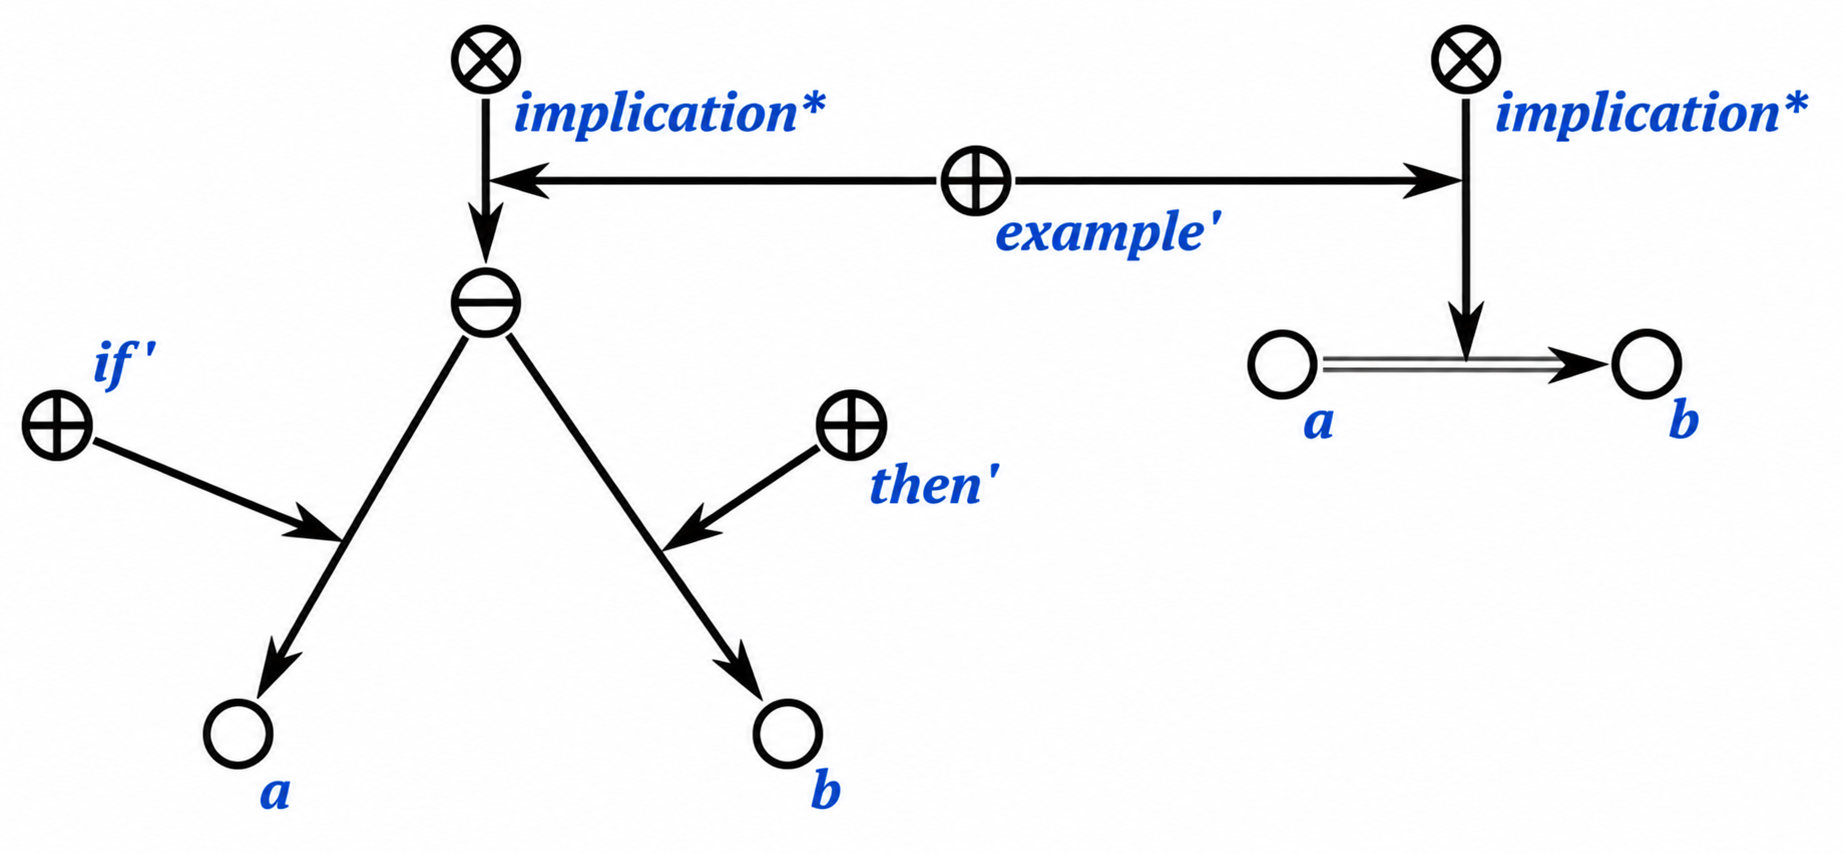
\includegraphics[width=339bp,height=156.75bp,keepaspectratio]{./figures/sd_logic/implication_en.png}
	\end{figure}
\end{frame}

\begin{frame}{\\Equivalence}
	\topline
	\justifying
	\footnotesize{
		\begin{SCn}
			\scnheader{equivalence connective*}
			\scnidtf{equivalence*}
			\scnsubset{logical connective*}
			\scniselement{binary relation}
			\scniselement{undirected relation}
			\scntext{explanation}{\textbf{\textit{equivalence connective*}} is a set of \textit{propositions} about equivalence, each of which is true within a \textit{formal theory} if and only if both its components are either true within the same \textit{formal theory} or false.

By default, all variables occurring in both parts of a proposition about \textbf{\textit{equivalence connective*}} (or at least one of the \textit{subformulas*} of each part) are implicitly bound by a \textit{universal quantifier*}, provided that these variables are not bound by another \textit{quantifier} that is specified explicitly.}
		\end{SCn}
	}
\end{frame}

\begin{frame}{\\Equivalence}
	\topline
	\justifying
	\vspace{10mm}
	\begin{figure}[H]
		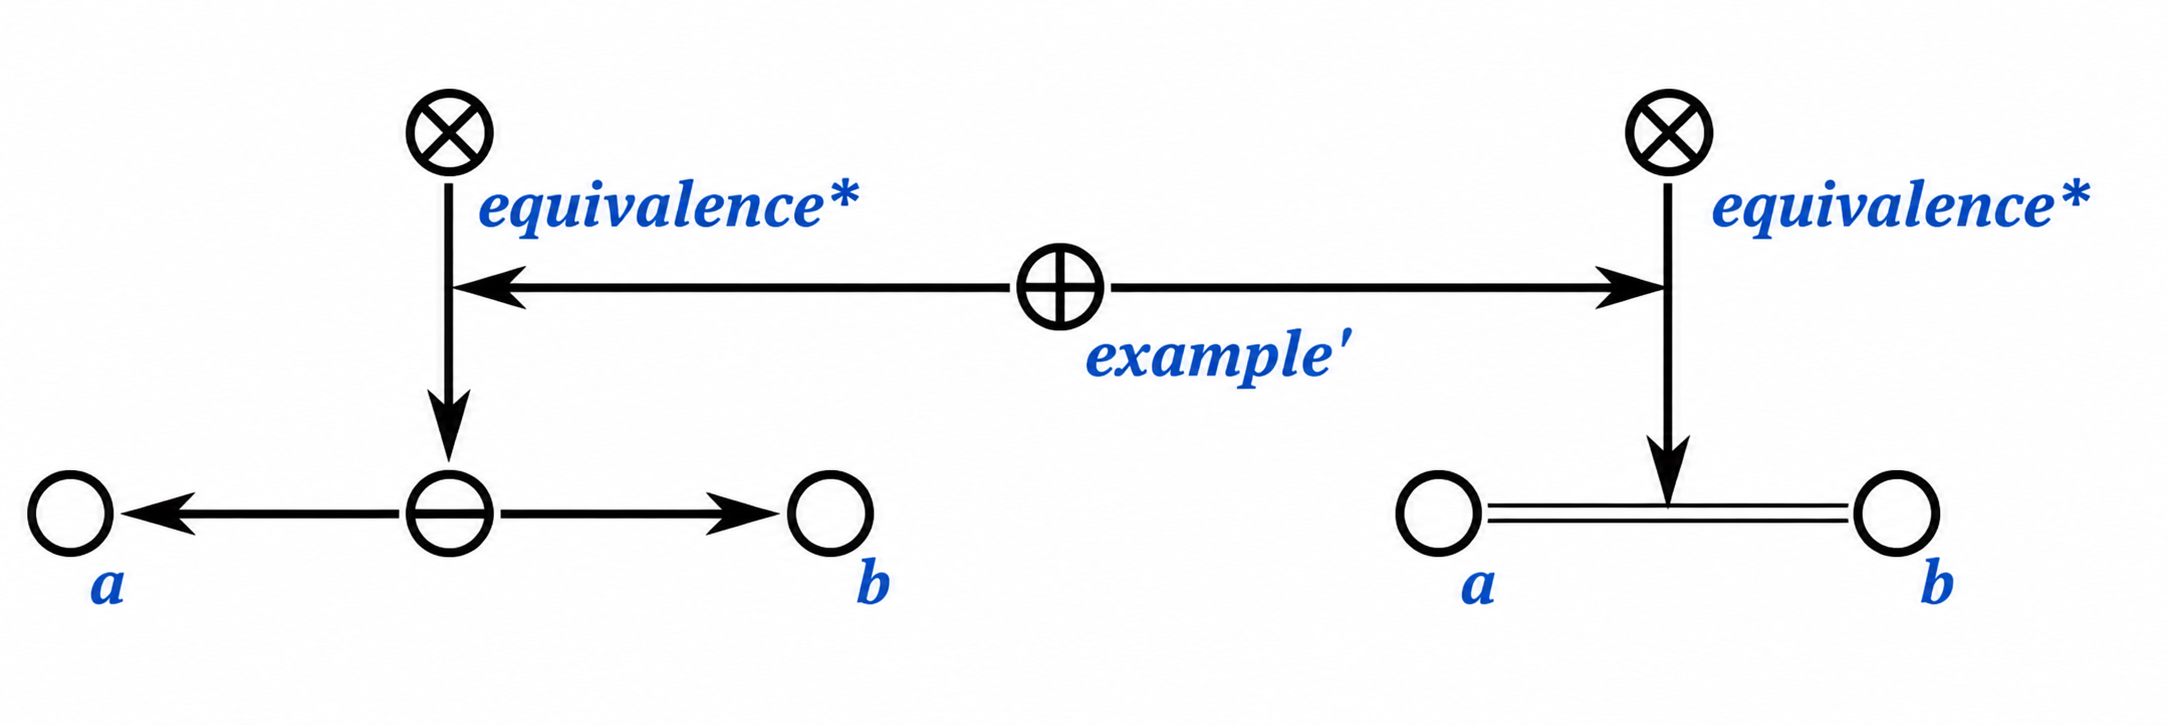
\includegraphics[width=321bp,height=89.25bp,keepaspectratio]{./figures/sd_logic/equivalent_en.png}
	\end{figure}
\end{frame}

\begin{frame}{\\ Truth tables of logical functions}
	\topline
	\justifying
	\vspace{5mm}
	\begin{center}
		\begin{tabular}{|c|c|c|c|c|c|c|c|}
			\hline
			$X$ & $Y$ & $\neg X$ & $X \land Y$ & $X \lor Y$ & $X \oplus Y$ & $X \to Y$ & $X \leftrightarrow Y$\\
			\hline
			$0$ & $0$ & $1$ & $0$ & $0$ & $0$ & $1$ & $1$\\
			\hline
			$0$ & $1$ & $1$ & $0$ & $1$ & $1$ & $1$ & $0$\\
			\hline
			$1$ & $0$ & $0$ & $0$ & $1$ & $1$ & $0$ & $0$\\
			\hline
			$1$ & $1$ & $0$ & $1$ & $1$ & $0$ & $1$ & $1$\\
			\hline
		\end{tabular}
	\end{center}
\end{frame}

\begin{frame}{\\Equivalence of logical formulas}
	\topline
	\\
	\footnotesize{
		Two logical formulas $A$ and $B$ are called equivalent if they have the same logical value for every combination of values of the elementary propositions (variables) occurring in them.\\
		\textit{Notation}: $A \iff B$
		\begin{center}
			\begin{tabular}{|c|c|}
				\hline
				$X \land X \iff X$ & $X \lor X \iff X$\\
				\hline
				$X \land \top \iff X$ & $X \lor \top \iff \top$\\
				\hline
				$X \land \bot \iff \bot$ & $X \lor \bot \iff X$\\
				\hline
				$X \land \neg X \iff \bot$ & $X \lor \neg X \iff \top$\\
				\hline
				$\neg(\neg X) \iff X$ & $X \lor (Y \land X) \iff X$\\
				\hline
				$X \land (Y \lor X) \iff X$ & $X \leftrightarrow Y \iff (X \leftarrow Y) \land (Y \leftarrow X)$\\
				\hline
				$X \leftarrow Y \iff \neg X \lor Y$ & $\neg(X \land Y) \iff \neg X \lor \neg Y$\\
				\hline
				$\neg(X \lor Y) \iff \neg X \land \neg Y$ & $X \land Y \iff \neg(\neg X \lor \neg Y)$\\
				\hline
				$X \lor Y \iff \neg(\neg X \land \neg Y)$ &\\
				\hline
			\end{tabular}
		\end{center}
	}
\end{frame}

\begin{frame}{\\De Morgan's laws}
	\topline
	\justifying
	\Huge
	\begin{center}
		$\neg(A \land B) \iff (\neg A \lor \neg B) $
		$\neg(A \lor B) \iff (\neg A \land \neg B) $
	\end{center}
\end{frame}

\begin{frame}{\\Tautology}
	\topline
	\justifying
	\begin{SCn}
		\scnheader{tautology}
		\scntext{explanation}{\textbf{\textit{tautology}} is a \textit{logical formula} that is either always true or always false within all \textit{formal theories} in which its truth or falsity can be established.

		\textbf{\textit{tautology}} is a \textit{logical formula} that is either a \textit{universally valid logical formula} or a \textit{contradictory logical formula}.}
	\end{SCn}
\end{frame}

\begin{frame}{\\Universally valid logical formula}
	\topline
	\justifying
	\begin{SCn}
		\scnheader{universally valid logical formula}
		\scnidtf{identically true logical formula}
		\scnsubset{consistent logical formula}
		\scnsubset{tautology}
		\scntext{explanation}{\textbf{\textit{universally valid logical formula}} is a \textit{logical formula} for which there is no \textit{formal theory} within which it would be false, given the truth and falsity of all its \textit{subformulas*} within that same \textit{formal theory}.}
	\end{SCn}
\end{frame}

\begin{frame}{\\Universally valid logical formula}
	\topline
	\justifying
	\vspace{10mm}
	\begin{figure}[H]
		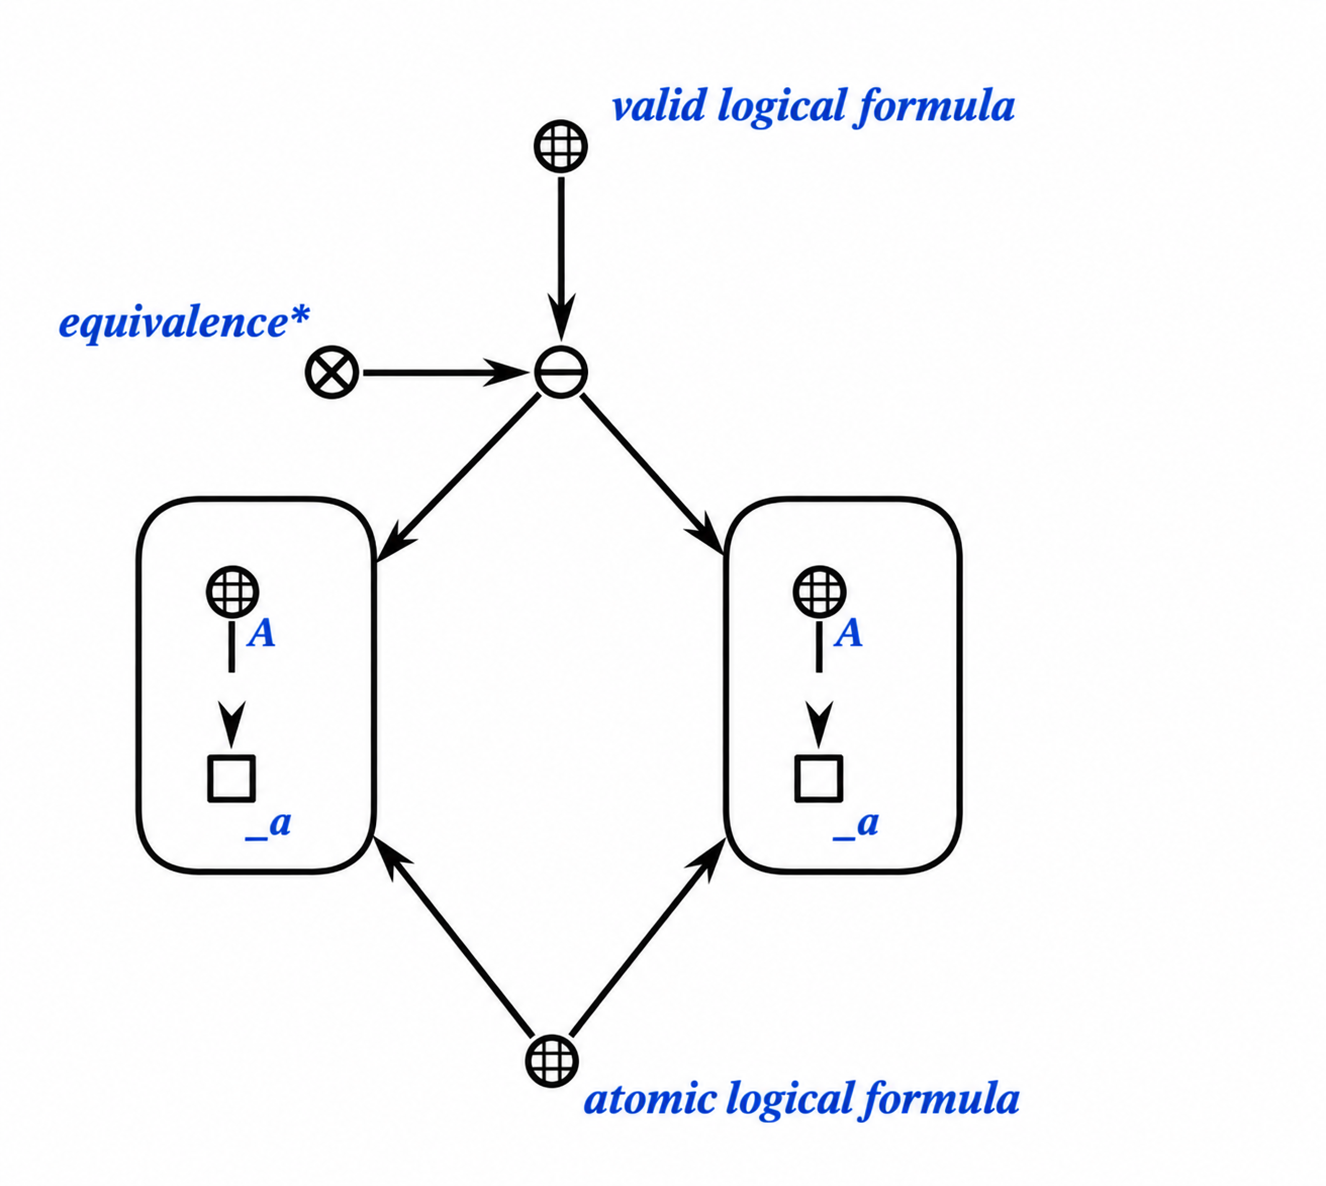
\includegraphics[width=202.8bp,height=181.35bp,keepaspectratio]{./figures/sd_logic/valid_formula_en.png}
	\end{figure}
\end{frame}

\begin{frame}{\\Contradictory logical formula}
	\topline
	\justifying
	\begin{SCn}
		\scnheader{contradictory logical formula}
		\scnidtf{identically false logical formula}
		\scnidtf{unsatisfiable logical formula}
		\scnsubset{tautology}
		\scntext{explanation}{\textbf{\textit{contradictory logical formula}} is a \textit{logical formula} for which there is no \textit{formal theory} within which it would be true, given the truth and falsity of all its \textit{subformulas*} within that same \textit{formal theory}.}
	\end{SCn}
\end{frame}

\begin{frame}{\\Contradictory logical formula}
	\topline
	\justifying
	\vspace{10mm}
	\begin{figure}[H]
		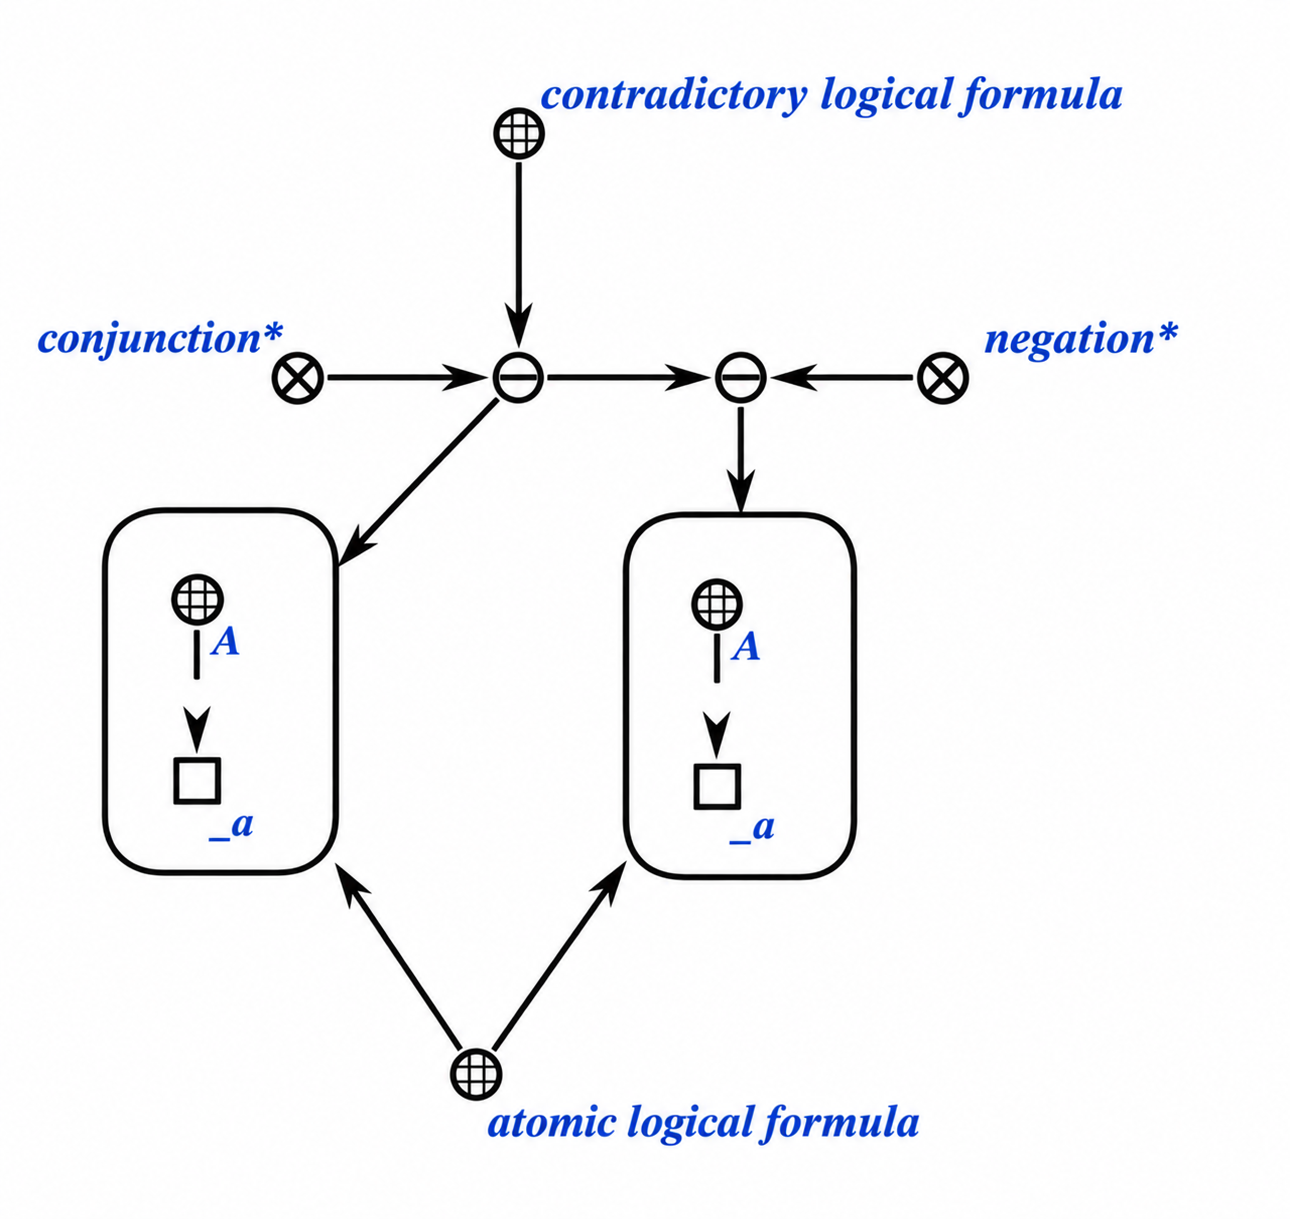
\includegraphics[width=177.938bp,height=168.188bp,keepaspectratio]{./figures/sd_logic/contradiction_formula_en.png}
	\end{figure}
\end{frame}

\begin{frame}{\\Contingent logical formula}
	\topline
	\justifying
	\begin{SCn}
		\scnheader{contingent logical formula}
		\scnsubset{consistent logical formula}
		\scntext{explanation}{\textbf{\textit{contingent logical formula}} is a \textit{logical formula} for which there is at least one \textit{formal theory} within which this formula is false, and at least one \textit{formal theory} within which this formula is true.}
	\end{SCn}
\end{frame}

\begin{frame}{\\Contingent logical formula}
	\topline
	\justifying
	\vspace{10mm}
	\begin{figure}[H]
		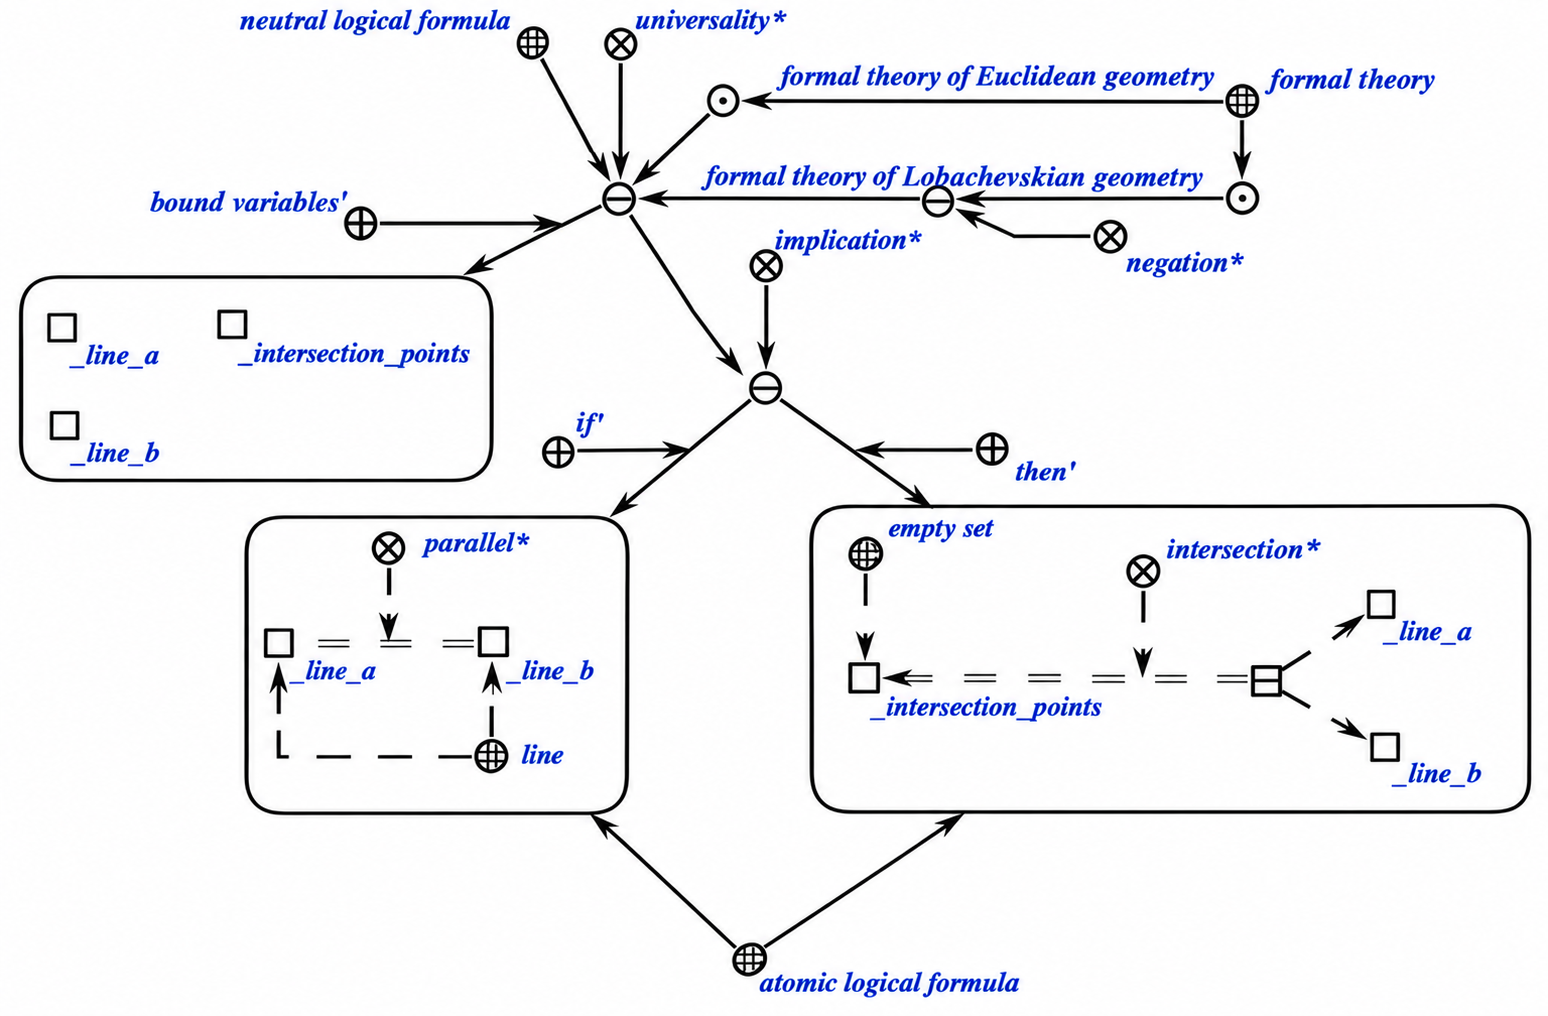
\includegraphics[width=270.675bp,height=177.863bp,keepaspectratio]{./figures/sd_logic/neutral_formula_en.png}
	\end{figure}
\end{frame}

\begin{frame}{\\Consistent logical formula}
	\topline
	\justifying
	\begin{SCn}
		\scnheader{consistent logical formula}
		\scnidtf{satisfiable logical formula}
		\scntext{explanation}{\textbf{\textit{consistent logical formula}} is a \textit{logical formula} for which there is at least one \textit{formal theory} within which this formula is true.}
		\begin{scnreltoset}{union}
			\scnitem{contingent logical formula}
			\scnitem{universally valid logical formula}
		\end{scnreltoset}
	\end{SCn}
\end{frame}

\begin{frame}{\\Non-valid logical formula}
	\topline
	\justifying
	\begin{SCn}
		\scnheader{non-valid logical formula}
		\scntext{explanation}{\textbf{\textit{non-valid logical formula}} is a \textit{logical formula} for which there is at least one \textit{formal theory} within which this formula is false.}
		\begin{scnreltoset}{union}
			\scnitem{contingent logical formula}
			\scnitem{contradictory logical formula}
		\end{scnreltoset}
	\end{SCn}
\end{frame}

\begin{frame}{\\Quantifier}
	\topline
	\justifying
	\begin{SCn}
		\scnheader{quantifier}
		\scnsubset{logical connective*}
		\scntext{explanation}{\textbf{\textit{quantifier}} is a \textit{relation}, each tuple of which specifies the truth of a set of \textit{logical formulas} contained in it, subject to additional conditions on some of the variables occurring in these \textit{logical formulas}.\\

We say that the variables are bound by a \textbf{\textit{quantifier}} or fall within the scope of that \textbf{\textit{quantifier}} (referring to a particular tuple of a particular \textbf{\textit{quantifier}}).\\

Each tuple of each \textbf{\textit{quantifier}} contains an \textit{atomic formula} that is a \textit{trivial structure} listing the variables bound by that \textbf{\textit{quantifier}}.}
	\end{SCn}
\end{frame}

\begin{frame}{\\Universal quantifier}
	\topline
	\justifying
	\footnotesize
	\vspace{10mm}
		\begin{SCn}
			\scnheader{universality*}
			\scnidtf{universal quantifier*}
			\scnidtf{universal quantification*}
			\scniselement{quantifier}
			\scniselement{directed relation}
			\scniselement{class of tuples of different cardinalities}
			\scntext{explanation}{\textbf{\textit{universality}} is a \textit{quantifier}, for each tuple of which that is true within a \textit{formal theory}, the following holds: all formulas contained in that tuple are true within the same \textit{formal theory} for all possible values of all elements of the set of \textit{bound variables\scnrolesign} contained in that tuple.

Each tuple of \textit{quantifier} \textbf{\textit{universality*}} can be represented as a \textit{conjunction*} (potentially infinite) of the original \textit{logical formulas} contained in that tuple, in each of which all \textit{bound variables\scnrolesign} are replaced with their possible values.

The quantifier \textbf{\textit{universal quantifier*}} is often denoted by ``$\forall$'' and read as ``for all''{}, ``for each''{}, ``for any''{} or ``all''{}, ``each''{}, ``any''.
			}
		\end{SCn}
\end{frame}

\begin{frame}{\\Universal quantifier}
	\topline
	\justifying
	\vspace{10mm}
	\begin{figure}[H]
		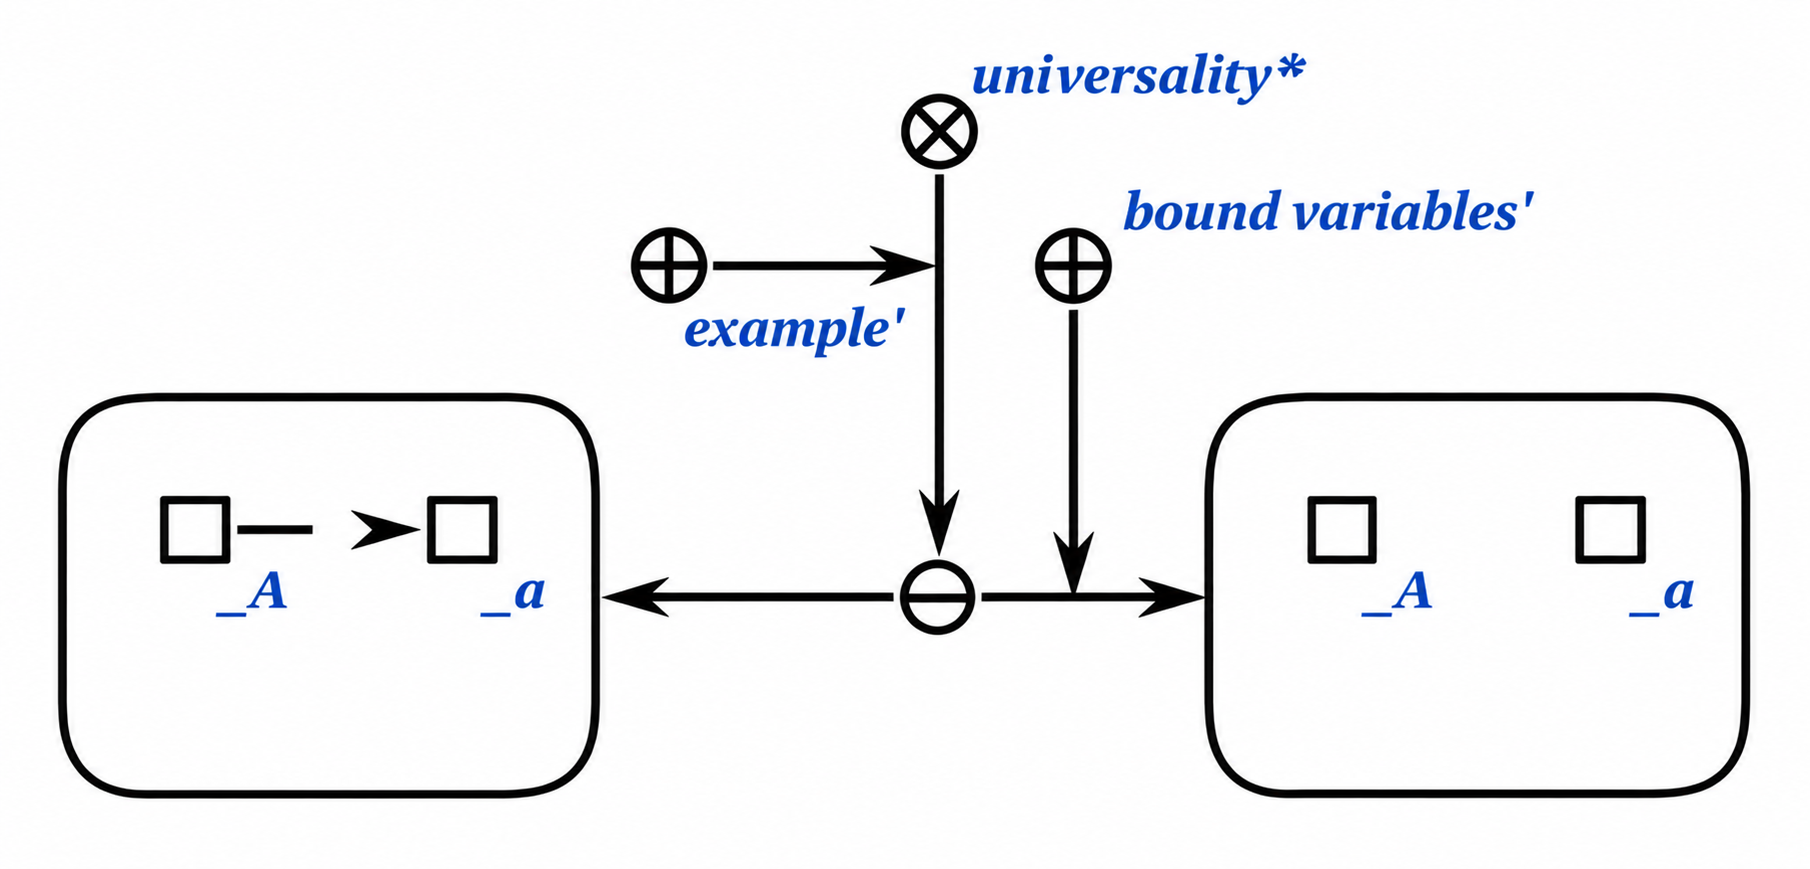
\includegraphics[width=304.5bp,height=146.25bp,keepaspectratio]{./figures/sd_logic/universality_en.png}
	\end{figure}
\end{frame}

\begin{frame}{\\Existential quantifier}
	\topline
	\justifying
	\begin{SCn}
		\scnheader{existence formula}
		\scnidtf{existence*}
		\begin{scnreltoset}{partition}
			\scnitem{atomic logical formula}
			\scnitem{non-atomic existence*}
		\end{scnreltoset}
	\end{SCn}
\end{frame}

\begin{frame}{\\Non-atomic existence}
	\topline
	\justifying
	\footnotesize{
		\begin{SCn}
			\scnheader{non-atomic existence*}
			\scnidtf{quantifier of non-atomic existence*}
			\scniselement{quantifier}
			\scniselement{directed relation}
			\scniselement{class of tuples of different cardinalities}
			\scntext{explanation}{\textbf{\textit{non-atomic existence*}} is a \textit{quantifier}, for each tuple of which that is true within a \textit{formal theory}, the following holds: there are values of all elements of the set of \textit{bound variables\scnrolesign} contained in that tuple such that all formulas in the tuple are true within the same \textit{formal theory}.

Each tuple of \textit{quantifier} \textbf{\textit{non-atomic existence*}} can be represented as a \textit{disjunction*} (potentially infinite) of the original \textit{logical formulas} contained in that tuple, in each of which all \textit{bound variables\scnrolesign} are replaced with their possible values.

The quantifier \textbf{\textit{existence*}} is often denoted by ``$\exists$'' and read as ``there exists''{}, ``for some''{}, ``there is''.}
		\end{SCn}
	}
\end{frame}

\begin{frame}{\\Non-atomic existence}
	\topline
	\justifying
	\vspace{10mm}
	\begin{figure}[H]
		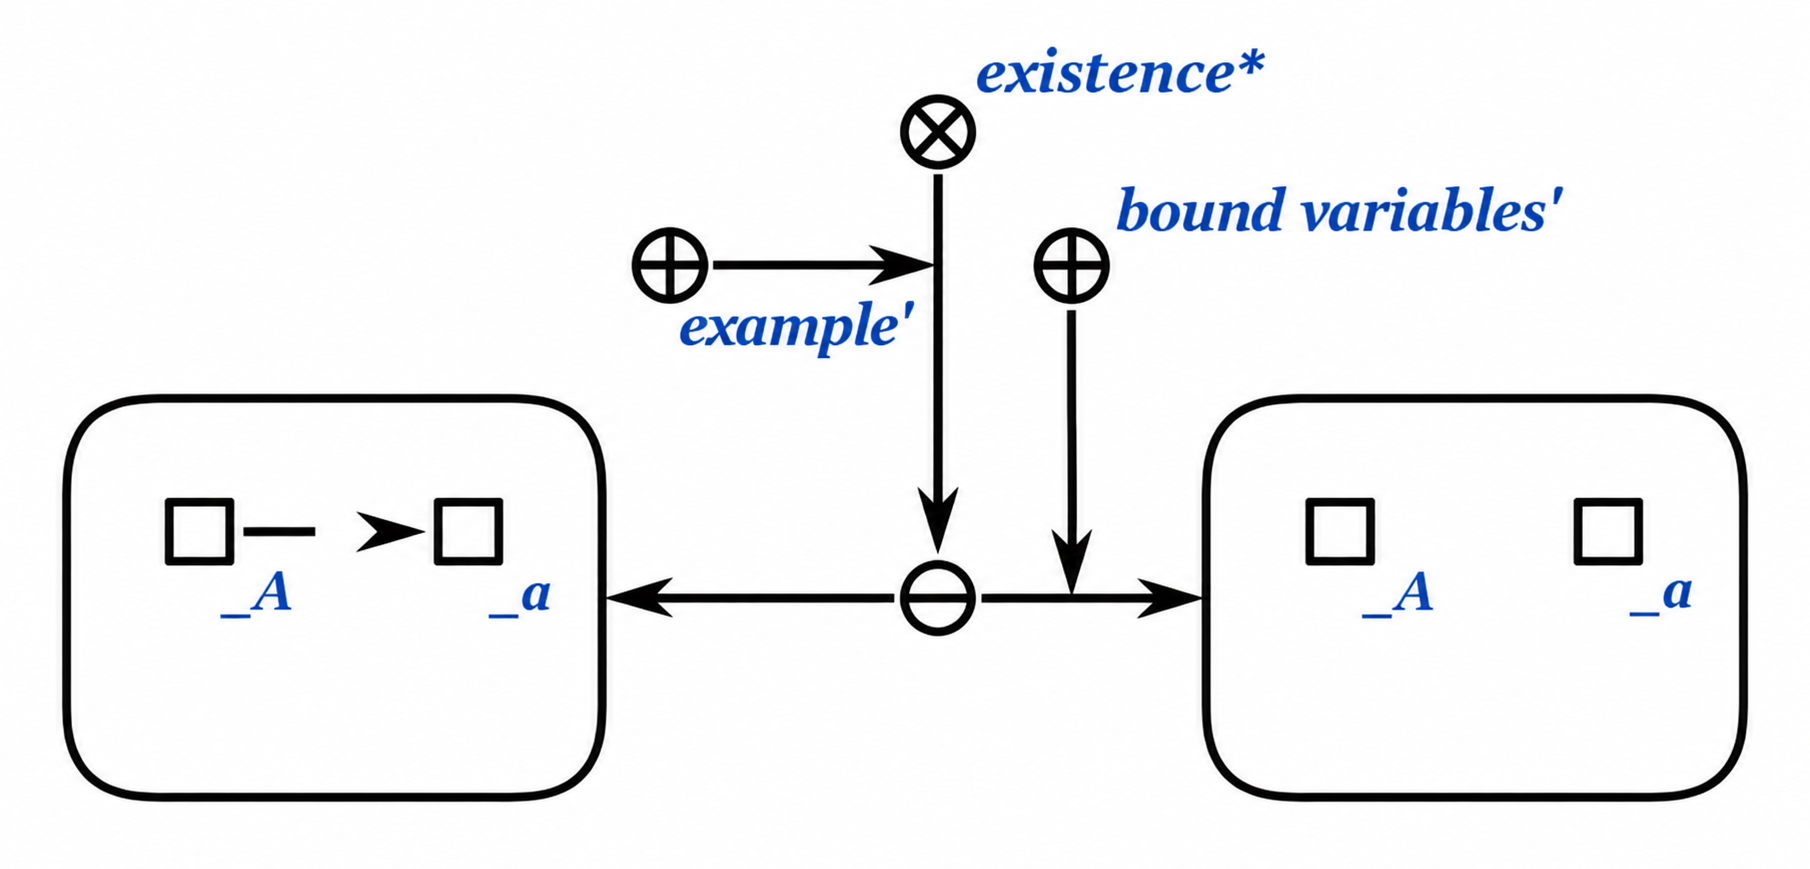
\includegraphics[width=304.5bp,height=146.25bp,keepaspectratio]{./figures/sd_logic/non_atomicExistence_en.png}
	\end{figure}
\end{frame}

\begin{frame}{\\Unique existence}
	\topline
	\justifying
	\begin{SCn}
		\scnheader{unique existence}
		\scnidtf{single existence}
		\scnidtf{existence and uniqueness formula}
		\scntext{explanation}{\textbf{\textit{unique existence}} is often denoted by ``$\exists!$\textquotedblright{} and is read as ``there exists exactly one''{}.}
	\end{SCn}
\end{frame}

\begin{frame}{\\Unique existence}
	\topline
	\justifying
	\begin{SCn}
		\scnheader{logical formula with uniqueness}
		\scnsubset{logical formula}
		\scnsubset{unique existence}
		\scntext{explanation}{Each \textbf{\textit{logical formula with uniqueness}} is a \textit{logical formula} (\textit{atomic} or \textit{non-atomic}) with the additional condition that, when interpreted over a subject domain, there is exactly one assignment of values to the variables in this formula (or its \textit{subformulas*}) for which the logical formula is true within the \textit{formal theory} containing the given \textit{subject domain}.}
	\end{SCn}
\end{frame}

\begin{frame}{\\Unique existence}
	\topline
	\justifying
	\vspace{10mm}
	\begin{figure}[H]
		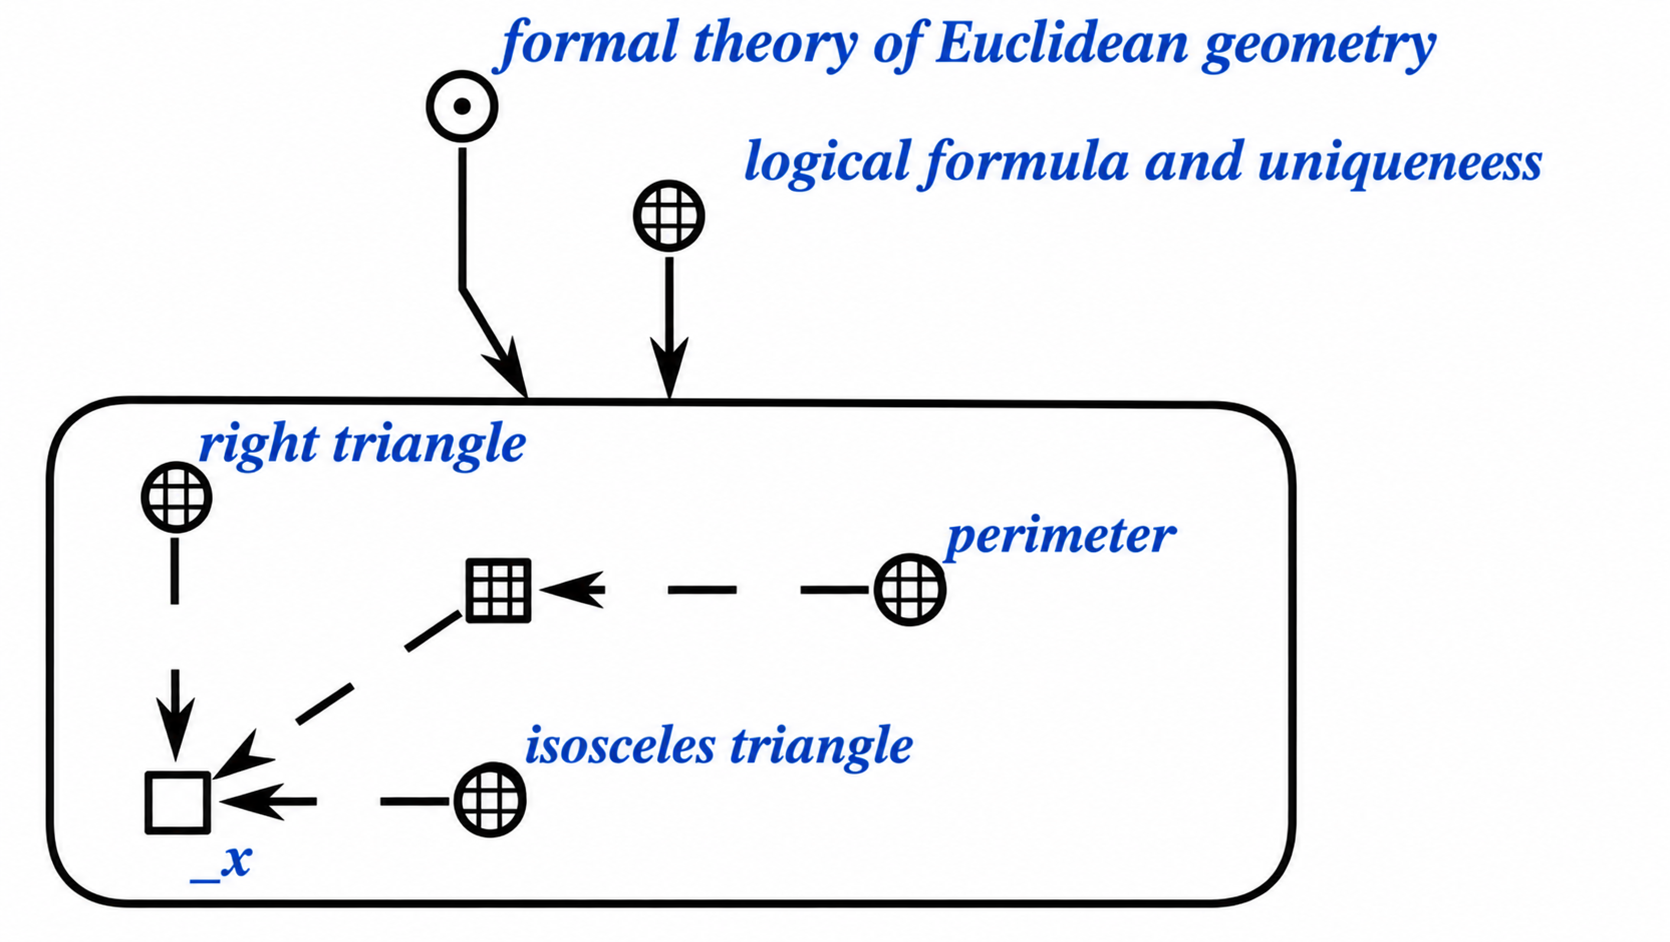
\includegraphics[width=297.75bp,height=168bp,keepaspectratio]{./figures/sd_logic/unique_existance_en.png}
	\end{figure}
\end{frame}

\begin{frame}{\\Duality of quantifiers}
	\topline
	\justifying
	\textbf{Duality} is a concept used in logic and mathematics whenever a one-to-one correspondence between two groups of concepts is established such that replacing the concepts of one group with the corresponding concepts of the other maps true propositions to true propositions.\\
Duality of quantifiers:
	\begin{center}
		$\neg(\forall xA(x)) \iff \exists x(\neg A(x))$\\
		$\neg(\exists xA(x)) \iff \forall x(\neg A(x))$
	\end{center}
\end{frame}

\begin{frame}{\\Bound variables}
	\topline
	\justifying
	\vspace{10mm}
	\footnotesize

		\begin{SCn}
			\scnheader{bound variables\scnrolesign}
			\scniselement{role relation}
			\scntext{explanation}{
				\textbf{\textit{bound variables\scnrolesign}} is a \textit{role relation} that relates a tuple of a particular \textit{quantifier} to the set of variables bound by that quantifier.
			}
			\scnheader{open logical formula}
			\scntext{explanation}{
				\textbf{\textit{open logical formula}} is a \textit{logical formula} within which (and all its \textit{subformulas*}) there is at least one variable that is not bound by any \textit{quantifier}.
			}
			\scnheader{closed logical formula}
			\scntext{explanation}{
				\textbf{\textit{closed logical formula}} is a \textit{logical formula} within which (and all its \textit{subformulas*}) there are no variables that are not bound by a \textit{quantifier}.
			}
		\end{SCn}
\end{frame}

\begin{frame}{\\Examples -- 1}
	\topline
	\justifying
	\Huge
	\begin{center}
	\begin{figure}[H]
		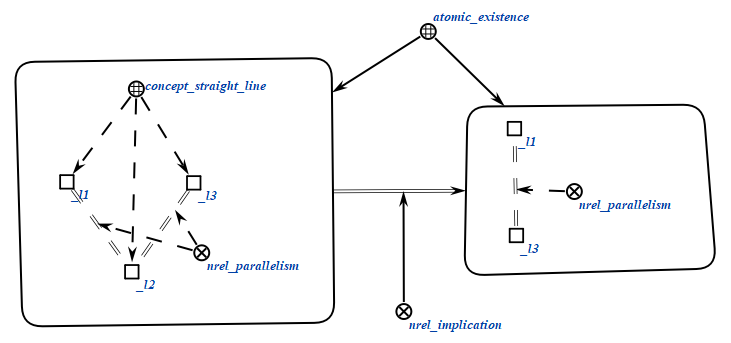
\includegraphics[scale=0.6]{./figures/sd_logic/example1.png}
	\end{figure}
	\end{center}
\end{frame}

\begin{frame}{\\Examples -- 2}
	\topline
	\justifying
	\Huge
	\begin{center}
	\begin{figure}[H]
		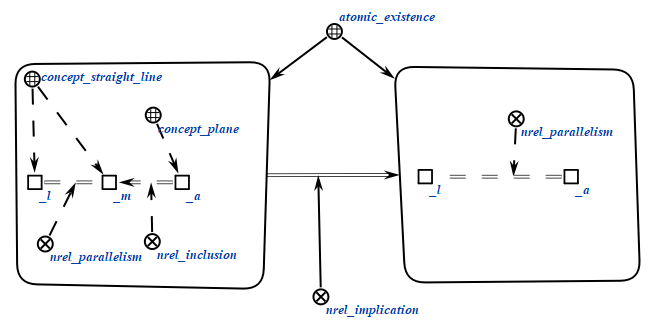
\includegraphics[width=0.94\linewidth,height=0.70\textheight,keepaspectratio]{./figures/sd_logic/example2.png}
	\end{figure}
	\end{center}
\end{frame}

\begin{frame}{\\Examples -- 3}
	\topline
	\justifying
	\Huge
	\begin{center}
	\begin{figure}[H]
		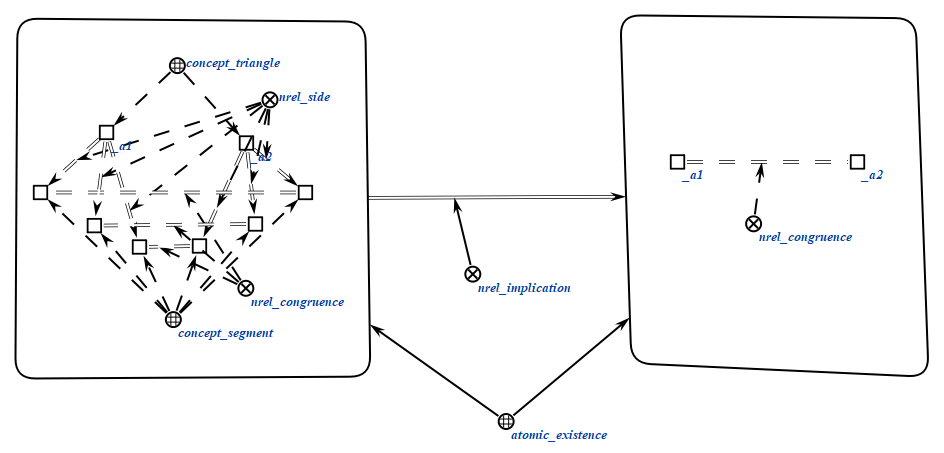
\includegraphics[width=0.94\linewidth,height=0.70\textheight,keepaspectratio]{./figures/sd_logic/example3.png}
	\end{figure}
	\end{center}
\end{frame}

\begin{frame}{\\Examples -- 4}
	\topline
	\justifying
	\Huge
	\begin{center}
	\begin{figure}[H]
		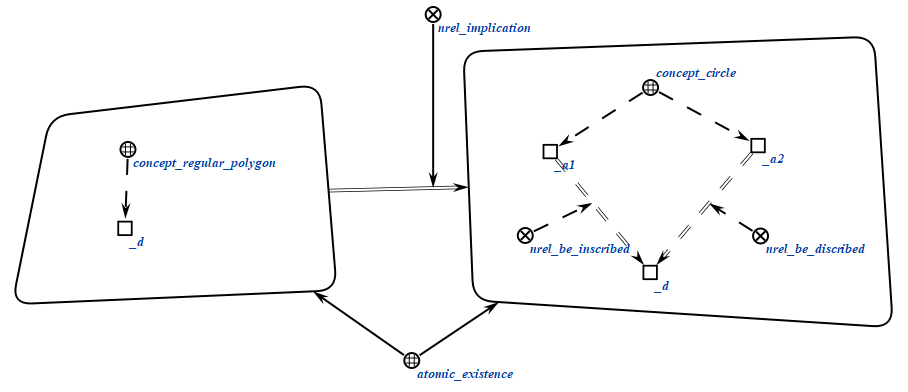
\includegraphics[width=0.94\linewidth,height=0.70\textheight,keepaspectratio]{./figures/sd_logic/example4.png}
	\end{figure}
	\end{center}
\end{frame}

\begin{frame}{\\Examples -- 5}
	\topline
	\justifying
	\Huge
	\begin{center}
	\begin{figure}[H]
		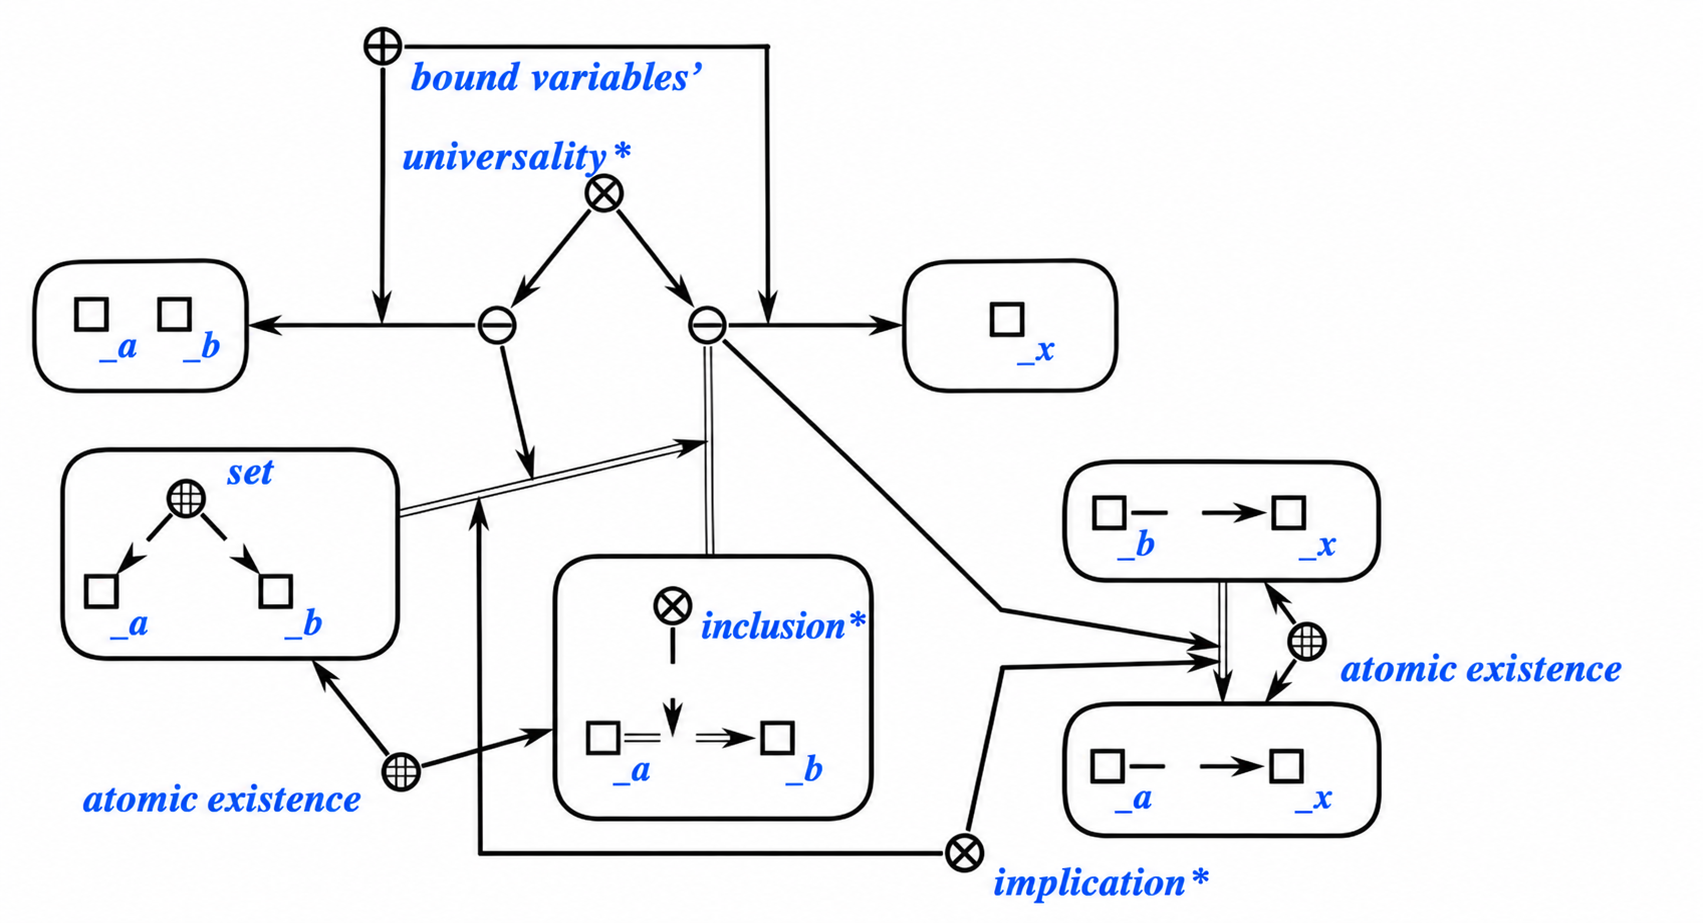
\includegraphics[width=340.2bp,height=184.5bp,keepaspectratio]{./figures/sd_logic/example5_en.png}
	\end{figure}
	\end{center}
\end{frame}
